\documentclass[../main.tex]{subfiles}
\begin{document}

Ein konkretes Beispiel Code der ein Sicherheitsrisiko darstellt und damit eventuell für nicht Compliance verantwortlich ist, ist die in Abbildung \ref{fig:codecompliance} dargestellte Funktion.

\begin{figure}[ht]
    \centering
    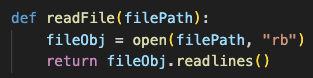
\includegraphics[scale=1]{bilder/CodeScreenShot.png}
    \caption{Python Risikocode, da eine geöffnete Datei nicht richtig geschlossen wird}
    \footnotesize (selbst geschrieben)
    
    \label{fig:codecompliance}
\end{figure}

In dem Beispiel wird mit Python eine Datei geöffnet und ihr Inhalt gelesen.
Die Datei wird allerdings nicht geschlossen.
Solche Fehler könnten zu unerwartetem Verhalten während der Laufzeit führen.
Deshalb müssen sie bereits davor erkannt werden.
Da eine Überprüfung per Hand fehleranfällig und langsam ist, braucht es hierfür eine Automatisierung.
Diese Automatisierung wird Check genannt.
\end{document}


